\documentclass{../lab_class}

\usepackage{fancyhdr}
\pagestyle{fancy}
\rhead{П.\,Ю. Смирнов, 687 гр.}
\lhead{Лабораторная работа № 4.6.1, МФТИ, весна 2018}

\begin{document}

{\Large 4.6.1 -- Интерференция электромагнитных волн миллиметрового диапазона.}

\paragraph{Цель работы.}
Изучение интерференции электромагнитных волн миллиметрового диапазона с применением двух оптических интерференционных схем, экспериментальное определение длины волны излучения и показателя преломления диэлектрика.

В работе используются: приёмно-передающая система радиоволн миллиметрового диапазона; металлические зеркала; микрометрический винт; проволочная решётка; пластина из диэлектрика.

\paragraph{Теоретическая часть.}
Для когерентных одинаково поляризованных волн с разностью фаз $\varphi$ мы знаем популярное выражение интенсивности суперпозиции:
\begin{equation}\label{eq:main}
	I = I_1 + I_2 + \sqrt{I_1 I_2} \cos \varphi,
\end{equation}
где разность фаз можно определить через разность хода волн: $\varphi = k \Delta$. Из \ref{eq:main} мы сразу легко объясним явление интерференции.

\begin{figure}[H]
	\centering
	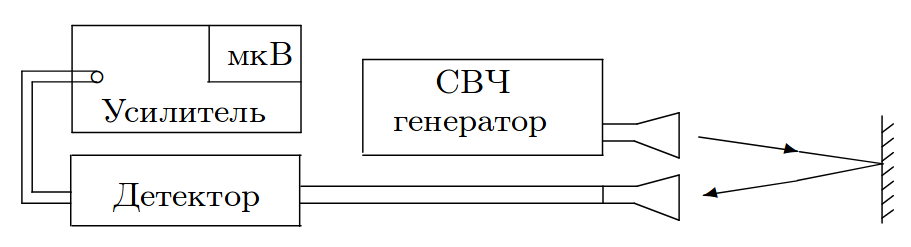
\includegraphics[width = 0.5 \textwidth]{sch01.png}
	\caption{Приёмно-передающая система СВЧ-диапазона.}
	\label{fig:sch01}
\end{figure}

На рис. \ref{fig:sch01} приведена схема используемой установки -- мы исследуем интерференцию СВЧ-волн; роль зеркала играет металлический лист. Прежде всего мы проверим \emph{закон Малюса}
\begin{equation}\label{eq:Malus}
	I = I_0 \cos^2 \alpha,
\end{equation}
где $\alpha$ -- поворот одной из антенн относительно луча. Выполнение данного закона свидетельствует о наблюдении линейно поляризованной волны.

\begin{figure}[H]
	\centering
	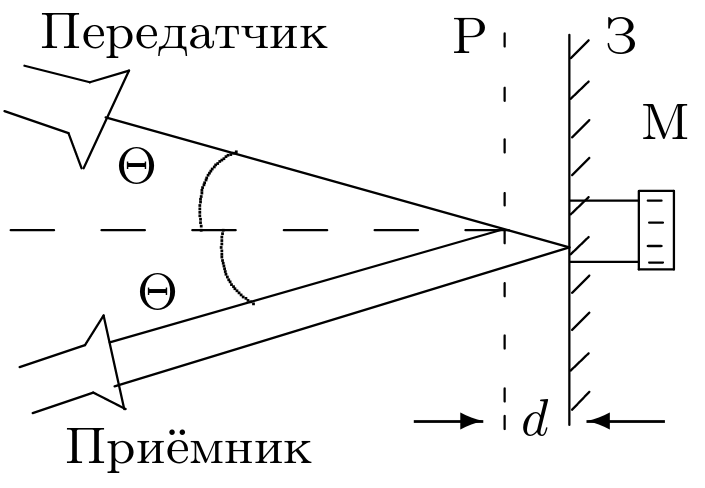
\includegraphics[width = 0.3 \textwidth]{sch02.png}
	\caption{Схема с зеркалом и решёткой для наблюдения интерференции радиоволн.}
	\label{fig:sch02}
\end{figure}

Если на расстоянии $d$ от зеркала поместить решетку (см. рис. \ref{fig:sch02}), частично отражающую волну, то можно наблюдать интерференцию радиоволн в приемнике. Разность хода даётся выражением
\begin{equation}\label{eq:lattice}
	\Delta = 2 d \cos \theta.
\end{equation}

Более того, мы можем собрать аналог оптического \emph{интерферометра Майкельсона} (см. рис. \ref{fig:sch03}). Разность хода возникает в результате разной длины плеч интерферометра: $\Delta = 2 (l_1- l_2)$. Если на пути одного из лучей поставить пластинку толщиной $h$ и диэлектрической пронициаемость $\varepsilon$, можно создать дополнительную разность хода $2 h (n-1)$. Пусть до внесения пластинки мы наблюдали интерференционный максимум. Тогда при сдвиге свободного плеча на $\delta x$ на расстояние
\begin{equation}\label{eq:Michelson}
	\delta x = h(n-1)
\end{equation}
мы будем снова наблюдать максимум. Если толщина пластинки настолько мала, что даваемая ей разность хода меньше длины волны света, то её показатель преломления может быть определен однозначно.

\begin{figure}[H]
	\centering
	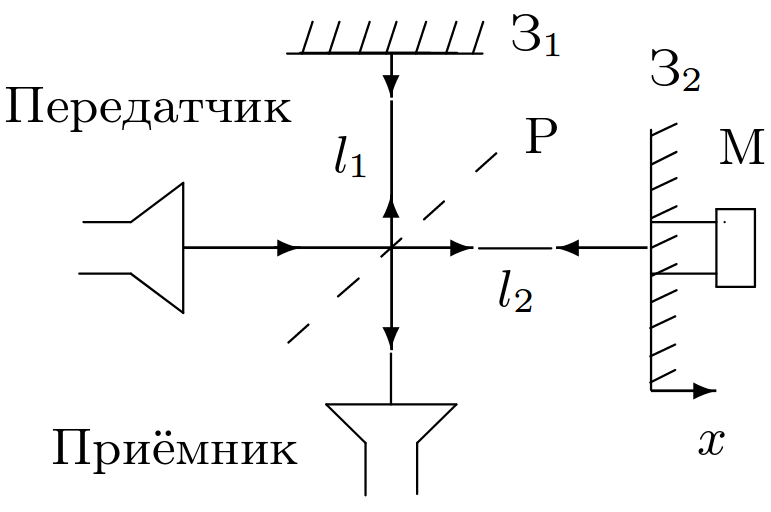
\includegraphics[width = 0.3 \textwidth]{sch03.png}
	\caption{Интерферометр Майкельсона на СВЧ-радиоволнах.}
	\label{fig:sch03}
\end{figure}

\paragraph{Проверка закона Малюса.}

Как видно по графику, закон выполняется.

\begin{center}
	\begin{tabular}{|c|c|c|c|c|c|c|}
		\hline
		$I, \smu \V$ & 26 & 24 & 21 & 18 & 14 & 10 \\ \hline
		$\alpha$  & 5 & 10 & 15 & 20 & 25 & 30 \\ \hline
	\end{tabular}
\end{center}

\begin{figure}[H]
	\centering
	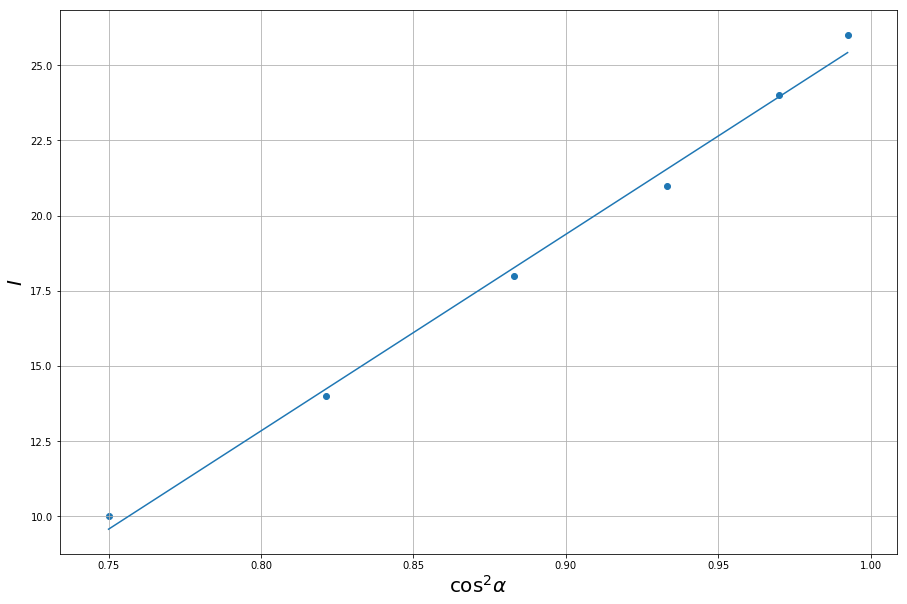
\includegraphics[width = 0.75 \textwidth]{pic01.png}
	\caption{Проверка закона Малюса.}
\end{figure}

\paragraph{Интерференция волн, отражённых от зеркала и решётки.}

100 делений -- 1 миллиметр. По графику находим, что расстояние между соседними максимумами есть $\simeq 4 \ \mm$;  согласно \ref{eq:lattice}  получаем экспериментально $\lambda \simeq 8 \ \mm$. При этом $\lambda = c / \nu \simeq 8.1 \ \mm$ -- истинное значение.

\begin{center}
	\begin{tabular}{|c|c|c|c|c|c|c|c|c|c|c|}
		\hline
		$I, \smu \V$ & 33 & 31 & 25 & 4 & 0 & 4 & 16 & 28 & 34 & 32 \\ \hline
		$x, \text{дел.}$ & 0 & 50 & 100 & 150 & 200 & 250 & 300 & 350 & 400 & 450 \\ \hline
	\end{tabular}
\end{center}

\begin{figure}[H]
	\centering
	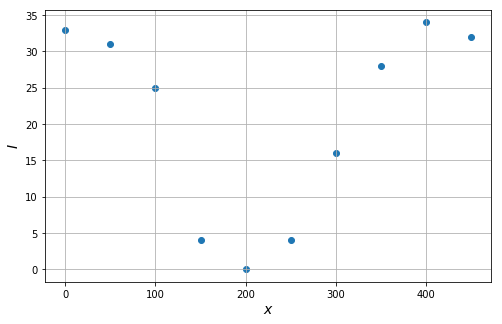
\includegraphics[width = 0.75 \textwidth]{pic02.png}
	\caption{Зависимость интенсивности от координаты подвижного зеркала.}
\end{figure}

\paragraph{Интерферометр Майкельсона.}
Перемещая подвижное зеркало, снимем зависимость координаты зеркала $x$ от номера максимума $n$. По графику определим длину волны: $2 \pi m = 2 \pi \Delta / x \then \lambda \simeq 7.34 \ \mm$.

\begin{center}
	\begin{tabular}{|c|c|c|c|c|c|c|}
		\hline
		$x, \ \mm$ & 3.72 & 7.69 & 11.8 & 15.78 & 19.7 & 23.8 \\ \hline
		$n$ & 1 & 2 & 3 & 4 & 5 & 6  \\ \hline
	\end{tabular}
\end{center}

\begin{figure}[H]
	\centering
	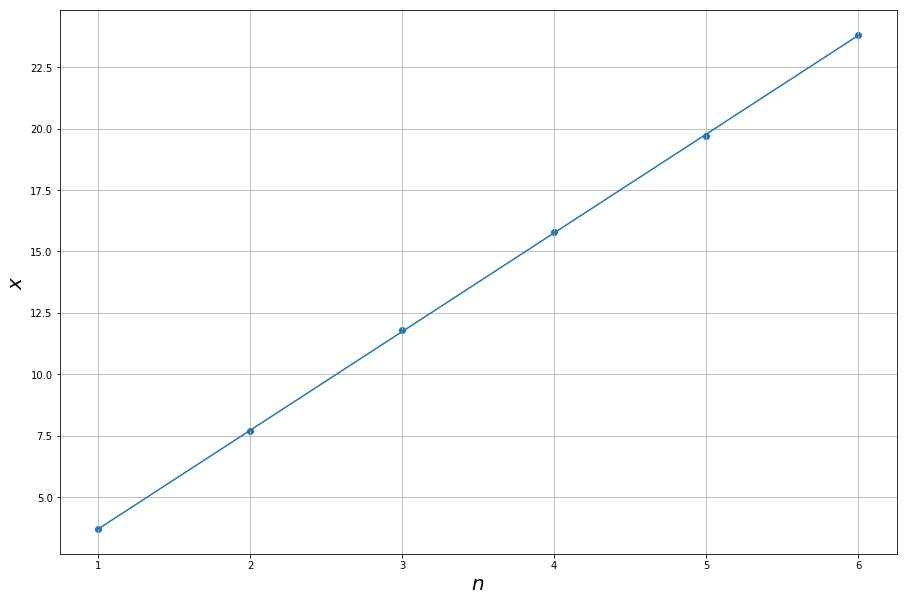
\includegraphics[width = 0.65 \textwidth]{pic03.png}
	\caption{Зависимость координаты зеркала $x$ от номера максимума $n$.}
\end{figure}

Найдем теперь зависимость $I = f(\Delta)$. Снимем зависимость интенсивности от координаты подвижного зеркала в пределах одной длины волны:
\begin{center}
	\begin{tabular}{|c|c|c|c|c|c|c|c|c|c|}
		\hline
		$I, \ \smu \V$ & 45 & 38 & 23 & 9 & 5 & 9.5 & 24 & 35 & 42 \\ \hline
		$x, \ \mm$ & 0 & 0.5 & 1 & 1.5 & 2 & 2.5 & 3 & 3.5 & 4 \\ \hline
	\end{tabular}
\end{center}

А теперь, убирая поочередно зеркала, измерим интенсивности каждого из интерферирующих лучей. Проверим, выполняется ли формула \ref{eq:main} (spoiler -- да).
\begin{center}
	\begin{tabular}{|c|c|c|c|c|c|c|c|c|c|}
		\hline
		$I, \ \smu \V$ & 44.9 & 39 & 24.7 & 10.6 & 5 & 11.2 & 25.7 & 39.7 & 44.9 \\ \hline
		$\Delta, \ \mm$ & 0 & 1 & 2 & 3 & 4 & 5 & 6 & 7 & 8 \\ \hline
	\end{tabular}
\end{center}

\begin{figure}[H]
	\centering
	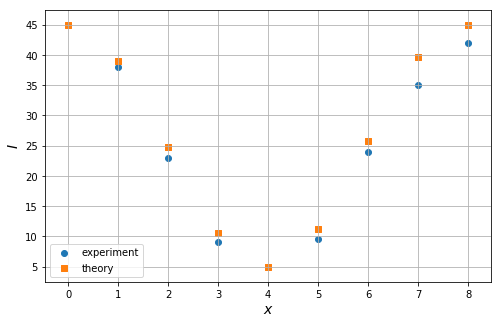
\includegraphics[width = 0.65 \textwidth]{pic04.png}
	\caption{Зависимость интенсивности от положения зеркала.}
\end{figure}

Ранее мы заметили, что в предположении малой толщины пластины мы можем легко найти её показатель преломления (см. формулу \ref{eq:Michelson}). У нас $\delta x \simeq 1 \ \mm \then n = 1 + \delta x / h \simeq 1.31$. Табличное значение -- $n = 1.4$.

\paragraph{Вывод.}
При исследовании интерференции СВЧ-волн мы проверили закон Малюса и получили замечательное согласие теории с опытом.

\end{document}









